% =====================================================================
% Allocation of the d_k/2 rotation planes of one attention head to
% physical coordinates.  Top strip: in the shared trunk and the mode
% branch every plane is rotated by the TOA t_n
% (\cref{eq:method:rope_block}).  Bottom strip: in the deinterleaving
% branch the planes are split evenly into two slices of d_k/4 planes,
% rotated by the horizontal direction components u^x_n and u^y_n
% (\cref{eq:method:rope_sliced}).  Loaded from
% sections/04_method/04_attention_variants.tex via \input{...}.
% =====================================================================
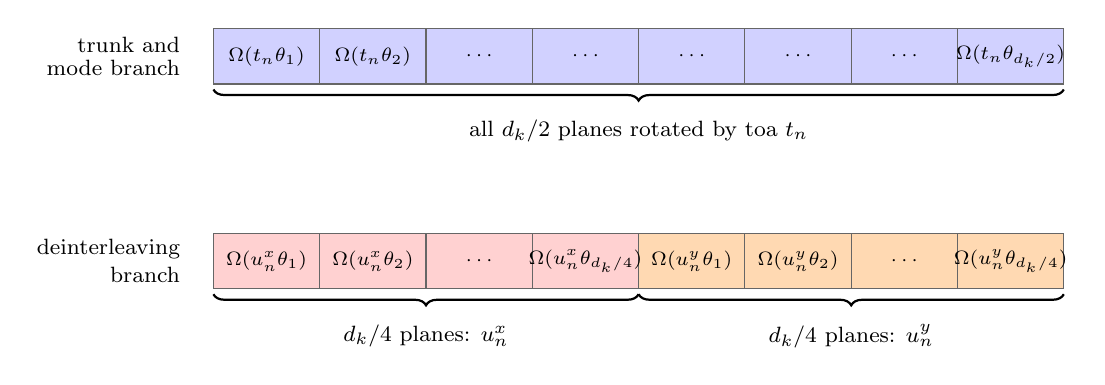
\begin{tikzpicture}[
    font=\small,
    plane/.style={draw=black!60, thin, minimum width=13.5mm, minimum height=7mm,
                  inner sep=0pt, outer sep=0pt},
    toaplane/.style={plane, fill=blue!18},
    uxplane/.style={plane, fill=red!18},
    uyplane/.style={plane, fill=orange!30},
    rowlabel/.style={font=\footnotesize, anchor=east},
    slicebrace/.style={decorate, decoration={brace, mirror, amplitude=4pt}, thick},
    bracelabel/.style={font=\footnotesize, anchor=north},
  ]

  \def\W{13.5mm}   % plane cell width
  \def\NP{8}    % number of plane cells drawn per strip

  % =================== TOP STRIP: trunk and mode branch =================
  \node[rowlabel] at (-3mm, 0) {\shortstack[r]{trunk and\\mode branch}};
  \foreach \m in {1,...,\NP} {
    \node[toaplane] (t\m) at ({(\m-0.5)*\W}, 0) {};
  }
  \node[font=\scriptsize] at (t1) {$\mat{\Omega}(t_n\theta_1)$};
  \node[font=\scriptsize] at (t2) {$\mat{\Omega}(t_n\theta_2)$};
  \node[font=\scriptsize] at (t3) {$\cdots$};
  \node[font=\scriptsize] at (t4) {$\cdots$};
  \node[font=\scriptsize] at (t5) {$\cdots$};
  \node[font=\scriptsize] at (t6) {$\cdots$};
  \node[font=\scriptsize] at (t7) {$\cdots$};
  \node[font=\scriptsize] at (t8) {$\mat{\Omega}(t_n\theta_{d_k/2})$};

  \draw[slicebrace] (0, -4.2mm) -- ({\NP*\W}, -4.2mm);
  \node[bracelabel] at ({\NP*\W/2}, -6.8mm)
    {all $d_k/2$ planes rotated by \gls{toa} $t_n$};

  % ============== BOTTOM STRIP: deinterleaving branch ====================
  \begin{scope}[yshift=-26mm]
    \node[rowlabel] at (-3mm, 0) {\shortstack[r]{deinterleaving\\branch}};
    \foreach \m in {1,...,4} {
      \node[uxplane] (b\m) at ({(\m-0.5)*\W}, 0) {};
    }
    \foreach \m in {5,...,8} {
      \node[uyplane] (b\m) at ({(\m-0.5)*\W}, 0) {};
    }
    \node[font=\scriptsize] at (b1) {$\mat{\Omega}(u^{x}_n\theta_1)$};
    \node[font=\scriptsize] at (b2) {$\mat{\Omega}(u^{x}_n\theta_2)$};
    \node[font=\scriptsize] at (b3) {$\cdots$};
    \node[font=\scriptsize] at (b4) {$\mat{\Omega}(u^{x}_n\theta_{d_k/4})$};
    \node[font=\scriptsize] at (b5) {$\mat{\Omega}(u^{y}_n\theta_1)$};
    \node[font=\scriptsize] at (b6) {$\mat{\Omega}(u^{y}_n\theta_2)$};
    \node[font=\scriptsize] at (b7) {$\cdots$};
    \node[font=\scriptsize] at (b8) {$\mat{\Omega}(u^{y}_n\theta_{d_k/4})$};

    \draw[slicebrace] (0, -4.2mm) -- ({4*\W}, -4.2mm);
    \node[bracelabel] at ({2*\W}, -6.8mm)
      {$d_k/4$ planes: $u^{x}_n$};

    \draw[slicebrace] ({4*\W}, -4.2mm) -- ({8*\W}, -4.2mm);
    \node[bracelabel] at ({6*\W}, -6.8mm)
      {$d_k/4$ planes: $u^{y}_n$};
  \end{scope}

\end{tikzpicture}
